\documentclass[titlepage]{article}

\usepackage[norsk]{babel}
\usepackage[T1]{fontenc}
\usepackage[utf8]{inputenc}

\usepackage{graphicx}
\usepackage{float}
\usepackage{url}
\usepackage{subfig}
\usepackage{listings}
\usepackage{verbatim}
\usepackage{SIunits}
\usepackage{multirow}
\usepackage{subfig}
\usepackage{hyperref}
\usepackage[hmargin=2cm,vmargin=2.5cm]{geometry}
\usepackage{listings}

\newcommand{\HRule}{\rule{\linewidth}{0.5mm}}
\usepackage[parfill]{parskip}

\begin{document}
%-----------------------------------------------------------
\begin{titlepage}
 
\begin{center}
 
\textsc{\LARGE TDT4225 Store Datamengder}\\[1.5cm]
\textsc{\Large Øving 1}\\[0.5cm]
 
\HRule \\[0.4cm]
{ \huge \bfseries Test av lesehastigheter}\\[0.4cm]
\HRule \\[1.5cm]

Trond Klakken \\
Elisabeth Solheim \\
Gunnar Inge Gjøvik Sortland

\vfill
 
% Bottom of the page
{\large \today}
 
\end{center}

\end{titlepage}

\section{Oppsett}
Vi har i dette forsøket målt lesetid for en fil på 1GB fra tre ulike
lagringsmedier.

Disse var Solid State disk (SSD) (\ref{SSD}), USB-minnepinne
(\ref{USB}) og fra ordinær disk (\ref{HDD}). For å sikre at hver test
ble uavhengig ble en fil på 1GB lest inn mellom hver av de, for å
flushe cache.

Testprogrammet kjører automatisk benchmarking for de 21 test
tilfellende gitt av oppgaven, og ble kjørt på hver av de tre mediene.

Grunnet mangel på tilgjengelig utstyr ble testene kjørt på to ulike
maskiner. Spesifikasjoner er gitt i tabell \ref{tab:hardware}. Dette
kan medføre at ulikheter i lesehastighet ikke bare skyldes mediet, men
også andre forhold. Trendene vi ser bør likevel være representive.

\begin{table}[h!]
 \caption{Benyttet maskinvare}
 \label{tab:hardware}
  \centering
  \begin{tabular}{|l|l|l|}
\hline
\textbf{Lagringsmedium} & \textbf{OS} & Filsystem \\
\hline
\hline
SDD & OSX & HFS+ \\
USB & OSX & FAT32 \\
HDD & Ubuntu & ext4 \\

\hline
\end{tabular}
\end{table}

\section{Resultater}

\begin{table}[h!]
\caption{Lesing av fil fra SSD OS (OSX)}
\label{SSD}
\centering
\begin{tabular}{|l|l|l|l|}
\hline
\multirow{2}{*}{ Antall parallelle delfiler} & \multicolumn{3}{|c|}{Blokkstørrelse} \\
 & 1024 & 4096 & 16384\\
\hline
1         &  0.211783  &  0.077320  & 0.048120 \\
2         &  0.214290  &  0.080882  & 0.049755 \\
4         &  9.423701  &  9.105014  & 1.996882 \\
8         & 11.315957  & 10.991903  & 3.694221 \\
16        & 11.201126  &  0.088839  & 0.054831 \\
32        &  6.082929  &  4.833985  & 1.345019 \\
tilfeldig &  0.557162  &  0.528545  & 0.455504 \\
\hline
\end{tabular}
\end{table}

\begin{figure}[h!]
  \caption{SDD}
  \label{fig:sdd}
  \centering
  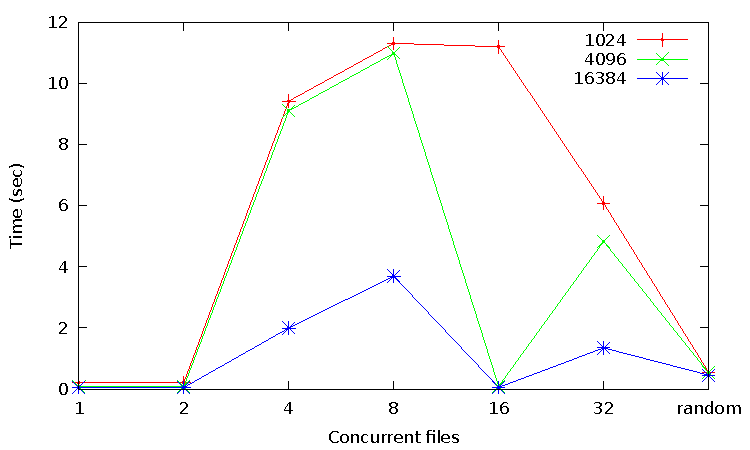
\includegraphics[width=0.5\textwidth]{res/result-sdd}
\end{figure}

\begin{table}[h!]
\caption{Lesing av fil fra USB minnepenn OS (OSX)}
\label{USB}
\centering
\begin{tabular}{|l|l|l|l|}
\hline
\multirow{2}{*}{ Antall parallelle delfiler} & \multicolumn{3}{|c|}{Blokkstørrelse} \\
 & 1024 & 4096 & 16384\\
\hline
1         &  16.234150 &   3.767864 &  3.344575 \\
2         &  20.408997 &  18.982415 &  0.663746 \\
4         &  37.190572 &  24.239117 &  4.832422 \\
8         &  37.350119 &  23.450713 &  8.085149 \\
16        &  37.177314 &  22.697717 &  7.437184 \\
32        &  36.742863 &  20.060136 &  6.026335 \\
tilfeldig &  16.653403 &   6.609872 &  8.190838 \\
\hline
\end{tabular}
\end{table}

\begin{figure}[h!]
  \caption{Plot of reading times using USB stick}
  \label{fig:usb}
  \centering
  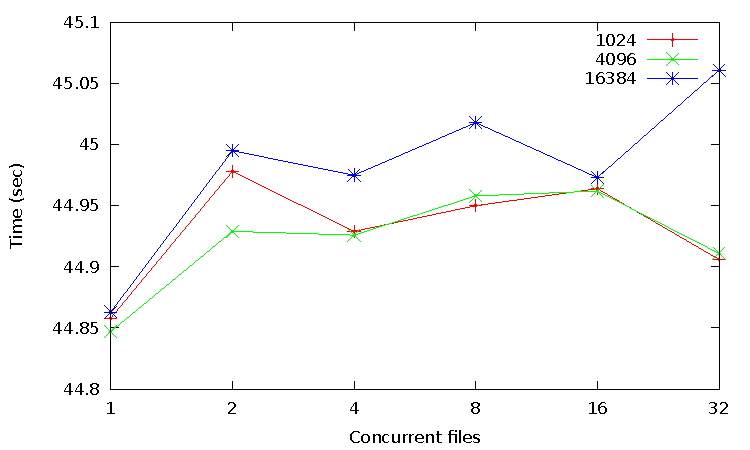
\includegraphics[width=0.5\textwidth]{res/result-usb}
\end{figure}

\begin{table}[h!]
\caption{Lesing av fil fra Harddisk (Linux)}
\label{HDD}
\centering
\begin{tabular}{|l|l|l|l|}
\hline
\multirow{2}{*}{ Antall parallelle delfiler} & \multicolumn{3}{|c|}{Blokkstørrelse} \\
 & 1024 & 4096 & 16384\\
\hline
1         &  0.164577 &  0.175946 & 0.078445 \\
2         &  0.162454 &  0.167318 & 0.080339 \\
4         &  0.165226 &  0.166446 & 0.075153 \\
8         &  0.167294 &  0.167608 & 0.074378 \\
16        &  0.167984 &  0.169632 & 0.080130 \\
32        &  0.172327 &  0.167756 & 0.076714 \\
tilfeldig &  8.910377 &  0.169295 & 4.817989 \\
\hline
\end{tabular}
\end{table}

\begin{figure}[h!]
  \caption{HDD}
  \label{fig:hdd}
  \centering
  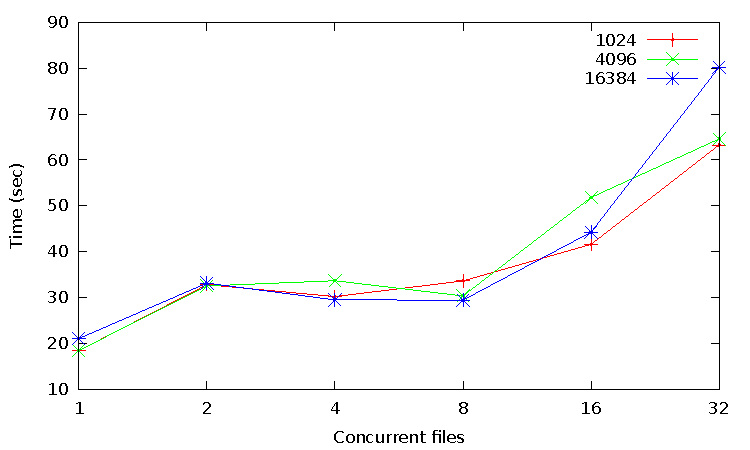
\includegraphics[width=0.5\textwidth]{res/result-hdd}
\end{figure}

Tabell \ref{SSD} og figur \ref{fig:sdd} viser kjøring ved SSD. Vi ser
en generell trend ved at økt blokkstørrelse gir lavere lesetid. Ved
økt antall parallelle åpne filer får vi noe høyere lesetid.

Lesing fra USB er, naturlig nok, veldig tregt som tabell \ref{USB} og
figur \ref{fig:usb} viser.

\section{Drøfting og konklusjon}
Ved bruk av SSD er søketiden relativt lav, slik at vi forventer at
dette ikke utgjør så mye som ved vanlig harddisk. Tabell \ref{HDD} og
figur \ref{fig:hdd} viser at dette ikke utgjør så mye som vi kunne
forvente.  På grunn av praktiske hensyn er det vanskelig å sammenligne
lesetid direkte, men trendene kan likevel sammenlignes.

Lesing via USB var, som nevnt, meget tregt.  Dette skyldes trolig at
overføringen er via USB og minnepennen var av billig modell.

Vi ser her at fra 4 til 32 parallelle filer påvirkes ikke
lesehastighet signifikant. Vi ser også her at større blokker gir
raskere lesing.

Lesing fra ordinær harddisk ble lite påvirket av antall parallelle
lesinger. Dette skyldes trolig god caching slik at søketid i stor grad
ble maskert. Vi ser likevel at ved lesing fra tilfeldig adresse øker
lesetiden veldig ved blokkstørrelse 1024 og 16384. Denne øker ikke ved
blokkstørrelse 4096, noe man forventer at skal skje.



\clearpage
\section{Appendix}

\clearpage
\subsection{\texttt{test.cpp} - Main program}
\lstinputlisting{../code/test.cpp}

\subsection{\texttt{Makefile}}
\lstinputlisting{../code/Makefile}

\clearpage
\subsection{\texttt{benchmark.h}}
\lstinputlisting{../code/benchmark.h}

\clearpage
\subsection{\texttt{benchmark.cpp}}
\lstinputlisting{../code/benchmark.cpp}

\end{document}
